% set 0 inch indentation
\setlength{\parindent}{0in} 
% set paragraph space = 1 space
\setlength{\parskip}{1em}
% set line space 1.5
\setlength{\baselineskip}{1.6em}

\chapter{Methodology}
\label{ch:methodology}
\paragraph{}
The main methodology of proposed study can be separated into four main processes as following and is shown in Figure \ref{fig:system_overview}:
\begin{enumerate}
\item Design and build filter, amplifier and embedded system for seismic sensor in order to  measure vibration
\item Collect normally event such as human activities
\item Build  anomaly detection models for detecting anomaly event as fall
\item Deploy this system in the real environment
\end{enumerate}

\begin{figure}[H]
  \centering
  \caption[The overview system architecture.]{\emph{The overview system architecture.}}\label{fig:system_overview}
  \includegraphics[scale = 0.4]{figures/system_overview.jpg}  
\end{figure}




\section{Data Collection}
\paragraph{}
To collect raw data, we need to build our own embedded system because in order to detect human fall, the system must have the ability to detect human activities and objective drop. And then, we have to build an algorithm for collecting the vibration signal as well.

\subsection{Hardware}
\paragraph{}
	There are 4 significant components as shown in Figure \ref{fig:hardware}. Each component has their own proposed.
    
 \begin{figure}[h]
  \centering
  \caption[The required hardware to receive raw data.]{\emph{The required hardware to receive raw data. \\}}\label{fig:hardware}
  \includegraphics[scale = 0.2]{figures/hardware.jpg}  
\end{figure}

\paragraph{}
Firstly, a seismic sensor or geophone in Figure \ref{fig:seismic}, A geophone is a device that converts ground vibration (velocity) into voltage. It has historically been passive analog devices and typically comprise a spring-mounted wire coil moving within the field of a case-mounted permanent magnet to generate an electrical signal. The reason that I decided to use this model (Geophone - SM-24) is because it has a small size similar to a coin and is easy to install just laying it on the ground. However, it cannot connect to the microcontroller directly because it can generate voltage up to $ 28.8 V / m/s$. Therefore, we have designed an embedded system to convert voltage into range $0 - 5$ Volts.

\begin{figure}[H]
  \centering
  \caption[A geophone SM-24 and its inside elements.]{\emph{A geophone SM-24 and its inside elements. \\Reprinted from its brochure }}\label{fig:seismic}
  \includegraphics[scale = 0.3]{figures/seismic.jpg}  
\end{figure}

\paragraph{}
Secondly, The analog circuit of filter \& amplifier , which is shown in Figure \ref{fig:analog_circuit}, has 4 significant component as a dc offset, a high-pass filter (HPF) followed by an amplifier with including low-pass filter (LPF). The dc offset is designed for setting the reference signal as $2.5 V$. The HPF is designed to filter any frequencies that are outside the frequency range of interest. It has an ideal cutoff frequency around $100 Hz$. The amplifier provides the high voltage gain around $200 V/V$ needed for preparing the data to be sampled at high resolution at the analog to digital converter (ADC). Lastly, the low-pass filter has cut-off frequency at $100 kHz$.

\begin{figure}[H]
  \centering
  \caption[An analog circuit which was designed to be suitable with human activity]{\emph{An analog circuit which was designed to be suitable with human activity.}}\label{fig:analog_circuit}
  \includegraphics[scale = 0.3]{figures/analogcircuit.jpg}  
\end{figure}

\paragraph{}
Thirdly, analog to digital converter (ADC), the higher bit means that it can contain more information. In Figure \ref{fig:adc}, you can get more intuitive what is the difference between 10-bit and 16-bit ADC.  The red line show the signal by using original adc pin on the Arduino mega which has only 10 bit and the blue line represent the signal by using 16-bit ADC. After the raw analog signal is filtered and amplified, it needs to be sampled at a rate of 500 samples/second and quantized at a resolution of 16 bits/sample in order to prepare it for digital transmission. A 16-bit ADC is capable of distinguishing $65536$ ($2^{16}$) different voltage levels within a narrow voltage range from $0 - 5$ Volts. It means that each level represents approximately $76.3 uV$ which is enough to capture signals of seismic sensor.

\begin{figure}[H]
  \centering
  \caption[This is different between 16-bit and 10-bit ADC.]{\emph{This is different between 16-bit and 10-bit ADC. }}\label{fig:adc}
  \includegraphics[scale = 0.3]{figures/ADC.jpg}  
\end{figure}

\paragraph{}
Fourthly, in Figure \ref{fig:pi4}, the used micro-computer is an Raspberry Pi 4 model B, which is a small size, low price, and several useful functions, and can do machine learning. The digital signal is fed from ADC to ESP8266 via I2C which is a synchronous serial communication interface specification used for short-distance communication. And then these raw signals  are directly collected into mircro sd card.

\begin{figure}[H]
  \centering
  \caption[Microcomputer - Raspberry Pi 4.]{\emph{Microcomputer - Raspberry Pi 4.}}\label{fig:pi4}
  \includegraphics[scale = 0.3]{figures/pi4.jpg}  
\end{figure}

\subsection{Experimental Setup}
\paragraph{}
To collect the raw data, experiments are performed in the living room of my house in Bangkok, Thailand which was built from reinforced concrete structure and on top with tile as show in Figure \ref{fig:home}. Actually, my system has detectable range around 3 meters and this room also has dimension 3.5 $x$ 3.5 $meter^2$. The hardware should be  installed near the corner in order to be as suitable for the application as possible.

\begin{figure}[H]
  \centering
  \caption[The living room where is used for experiment]{\emph{The living room where is used for experiment.}}\label{fig:home}
  \includegraphics[scale = 0.2]{figures/home.jpg}  
\end{figure}

\subsection{Experimental Event}
\paragraph{}
There are several events which should occur during the daily event. However, the author would like to only collect often activities such as walking, sitting, standing and lying as shown in Table \ref{tab:number_action}. Sincerely, due to covid-19 situation, I cannot invite strange volunteers to come in my house in order to collect data. However, If the covid situation in Thailand is better, I will invite approximate 5 - 10 friends to join this experimental event. Therefore, I plan to collect these activity with 4 subjects who are family member as my father, my mother, my older brother and me, and the detail of them is shown in Table \ref{tab:participants}.

\begin{table}[H]
\begin{center}
\caption[The detail of each activity and its number of action.]{\emph{The detail of each activity and its number of action.} \\ \hspace{\textwidth}}\label{tab:number_action}
\begin{tabular}{ l r }
  \textbf{Human Activity} & \textbf{Number of action}\\
\hline
Walking & 2,500 \\
\hline
Sitting & 400 \\
\hline
Standing & 400 \\
\hline
Lying & 400 \\
\hline
   \end{tabular}
\end{center}
 \end{table}
 
\begin{table}[H]
\begin{center}
\caption[The detail of each participant and their details.
]{\emph{The detail of each participant and their details.} 
\\ \hspace{\textwidth}}\label{tab:participants}
\begin{tabular}{c c c c}
  \textbf{Subject} & \textbf{Sex} &  \textbf{Age} & \textbf{Weight $(kg)$}  \\
\hline

1 & M & 23  & 58 \\
\hline

2 & M & 25  & 70 \\
\hline

3 & M & 55  & 70 \\
\hline

4 & F & 58  & 75 \\
\hline

   \end{tabular}
\end{center}
 \end{table}
 
\section{Anomaly Detection Models}
\paragraph{}
I choose two candidate models as autoencoder with LSTM architecture in Figure \ref{fig:LSTM_metho} and Transformer in Figure \ref{fig:transformer_metho} , which are quite distinguished in this field.

\begin{figure}[H]
  \centering
  \caption[The autoencoder with LSTM architecture.]{\emph{The autoencoder with LSTM architecture}}\label{fig:LSTM_metho}
  \includegraphics[scale = 0.2]{figures/LSTM_metho.jpg}  
\end{figure}

\begin{figure}[H]
  \centering
  \caption[The Transformer architecture.]{\emph{The Transformer architecture. \\ Reprinted from work of \citeauthor{vaswani_shazeer_parmar_uszkoreit_jones_n_gomez_kaiser_polosukhin_2017} \citeyear{vaswani_shazeer_parmar_uszkoreit_jones_n_gomez_kaiser_polosukhin_2017}}}\label{fig:transformer_metho}
  \includegraphics[scale = 0.3]{figures/transformer_metho2.jpg}  
\end{figure}

 
\subsection{Evaluation Plan}
\paragraph{}
To assess the performance of the model, The model will be tested with untrained activities such as jumping and dropping the ball in different locus around the installed system. The prefered accuracy should be greater than 75 percents of true positive and 100 percents of true negative. (Not sure may be the number need to be changed)

\section{Deployment}
\paragraph{}
The desirable system should be plug \& play. Therefore, every component such as seismic sensor, embedded system and Raspberry Pi must be integrated into the small box, which require only power adapter as shown in Figure \ref{fig:application}. When anomaly activities are occuring, an alert messages is going to be sent via Line application to me. The dining room in my house will be the tested location of this study shown in \ref{fig:dining}.

\begin{figure}[H]
  \centering
  \caption[The complete application.]{\emph{The complete system.}} \label{fig:application}
  \includegraphics[scale = 0.5]{figures/application.png}  
\end{figure}

\begin{figure}[H]
  \centering
  \caption[The dining room in my home.]{\emph{The dining room in my home.}} \label{fig:dining}
  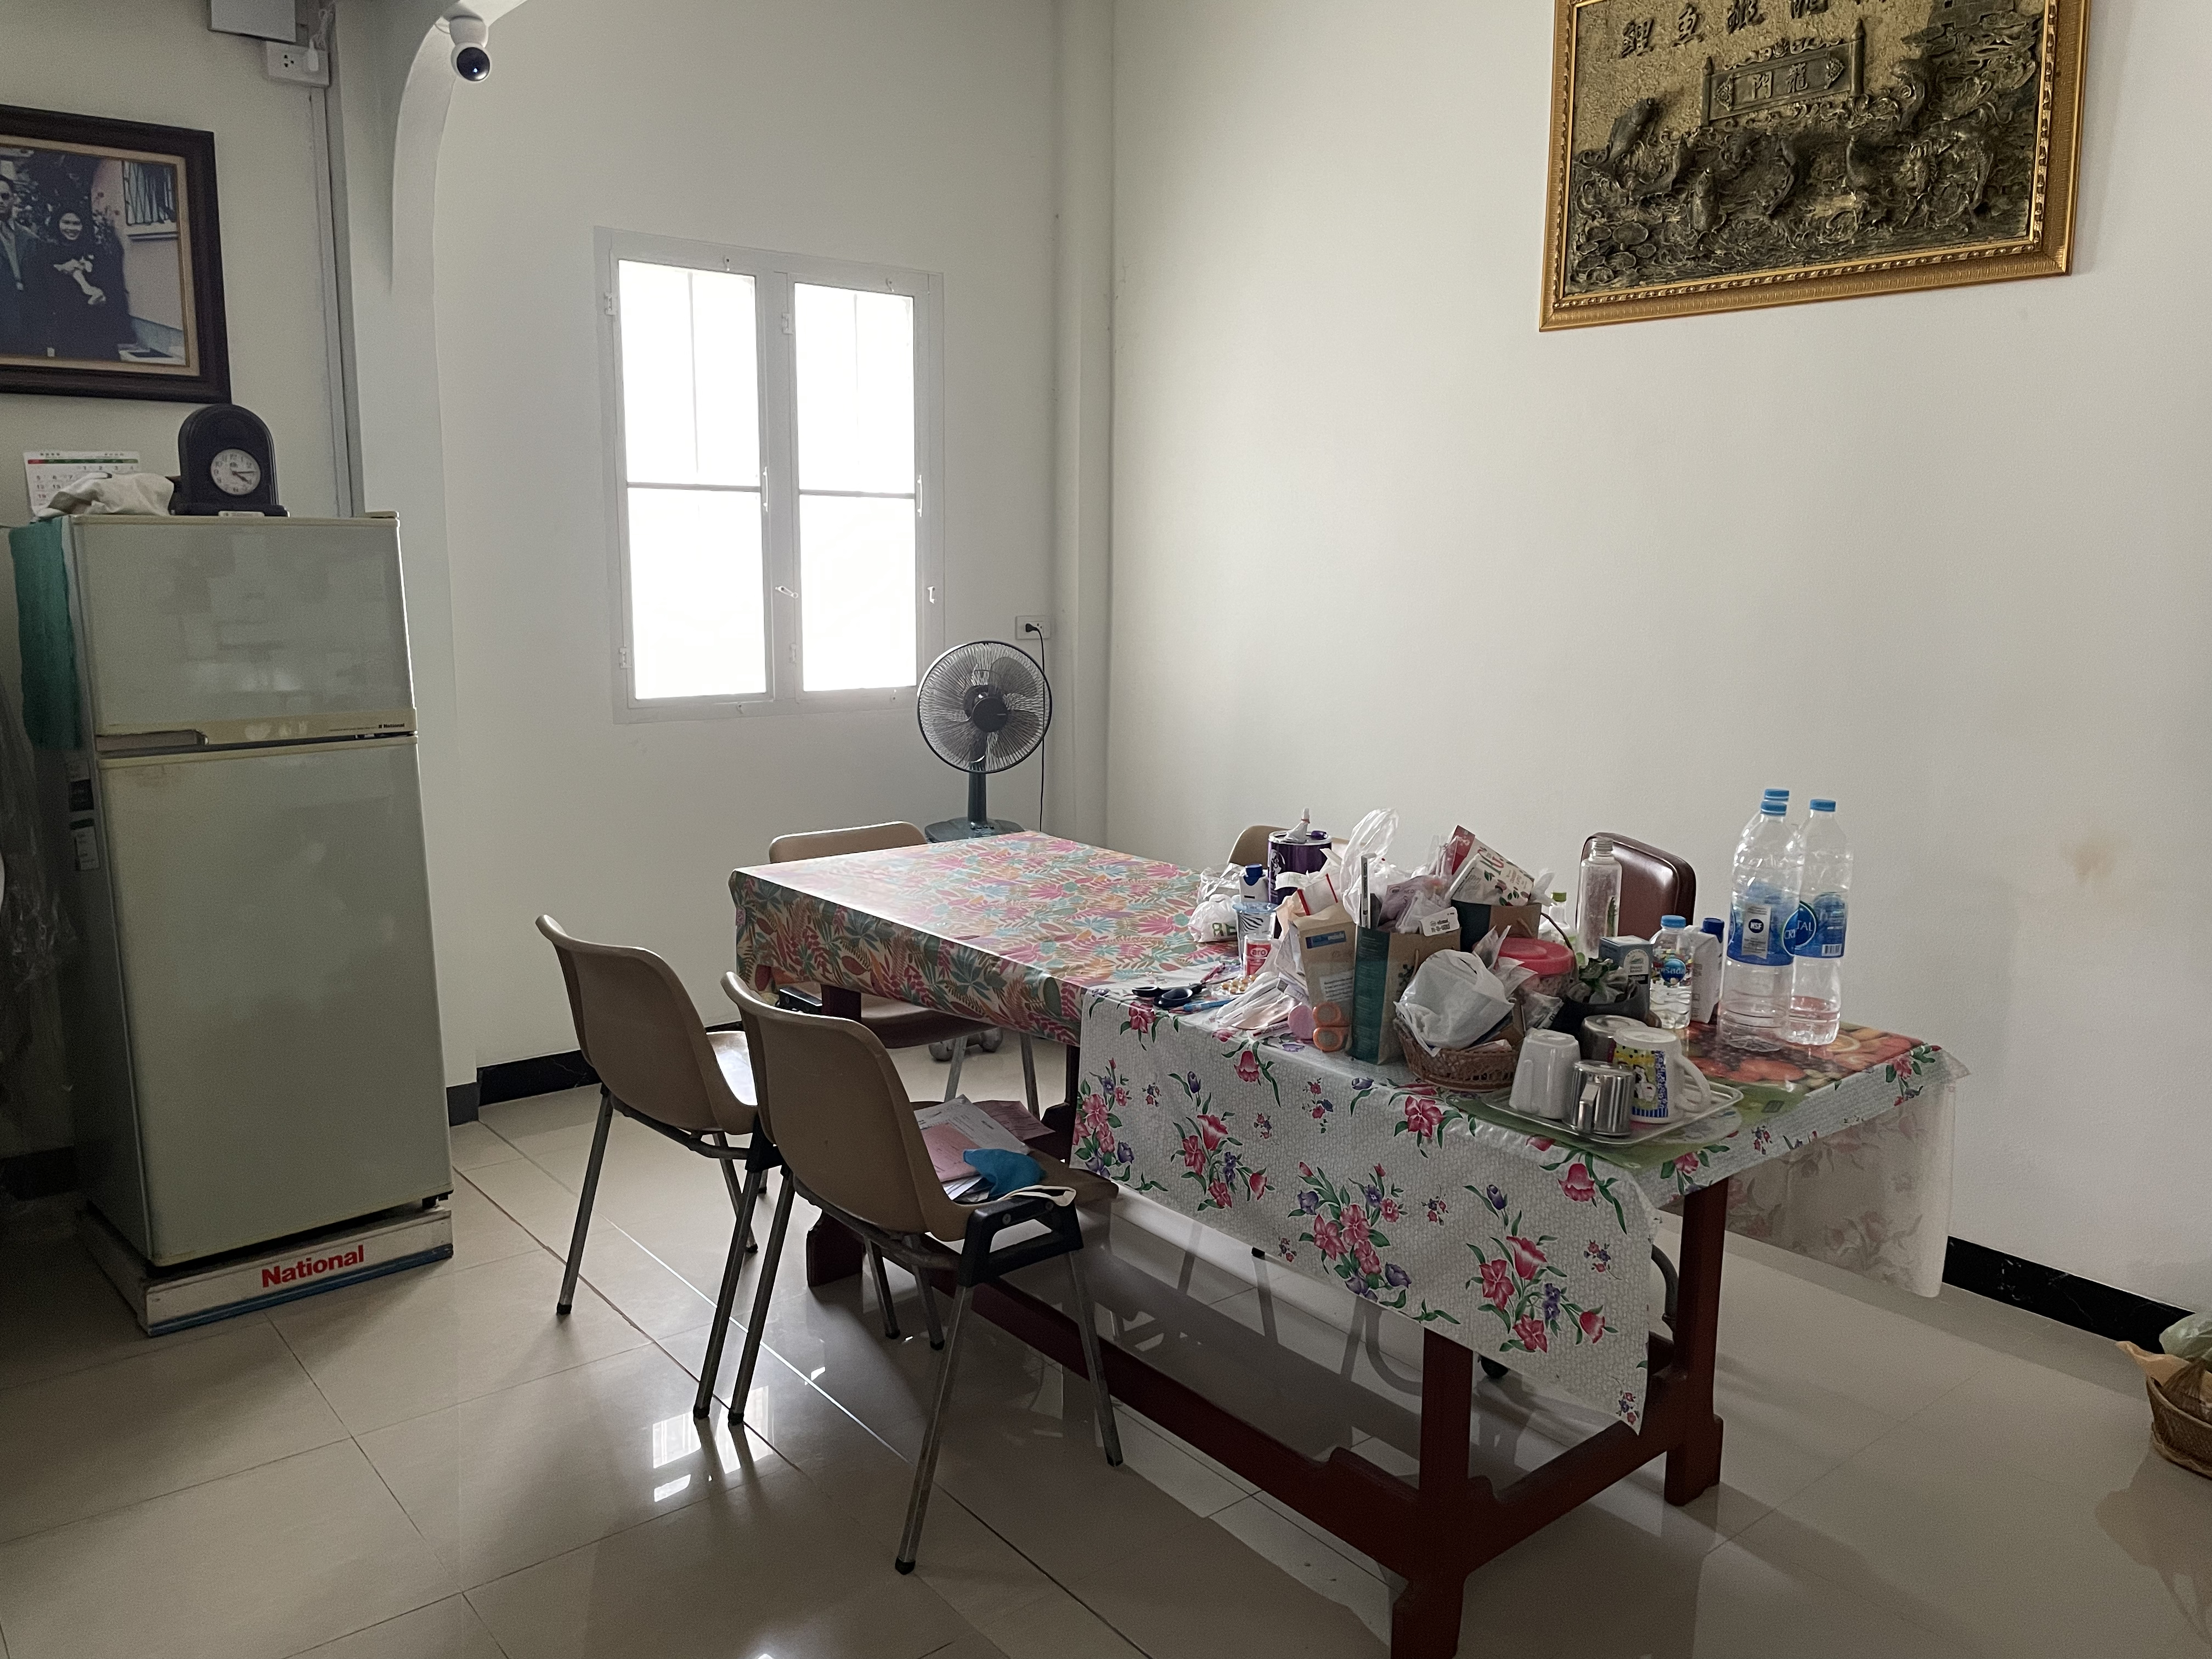
\includegraphics[scale = 0.1]{figures/dining.jpg}  
\end{figure}

\FloatBarrier